\documentclass[12pt]{report}
\usepackage{graphicx}
\usepackage{geometry}
\usepackage[italian]{babel}
\usepackage{xcolor}
\usepackage{float}
\usepackage{amssymb}
\usepackage{amsmath}
\usepackage{listings}
\usepackage{color}
\usepackage[utf8]{inputenc}
\usepackage{array}
\usepackage{longtable}
\usepackage{float}
\usepackage[hidelinks]{hyperref}
\usepackage{pgfplots}
\usepackage{fancyhdr}
\pagestyle{fancy}
\graphicspath{{images/}}

\geometry{a4paper, left=2cm, right=2cm, top=3cm}

% remove 'Chapter N'
\usepackage{titlesec}
\titleformat{\chapter}[display]
  {\normalfont\bfseries}{}{0pt}{\Huge}

% bibliography/links
\usepackage[
	backend=biber,
	style=draft,
]{biblatex}
\addbibresource{links.bib}

% custom fields for cover page
\usepackage{titling}
\pretitle{\begin{center}\placetitlepicture\Huge}
\posttitle{\par\lineskip 1em\placesubtitle\end{center}\vskip 3em}
\preauthor{\begin{center}
		\large \lineskip 3em%
		\begin{tabular}[t]{c}}
\postauthor{\end{tabular}\par\placecourse\par\placeprofessor\end{center}}
\predate{\begin{center}\large\vskip 3em}
\postdate{\par\placeversion\par\end{center}}

% commands for including the picture
\newcommand{\titlepicture}[2][]{%
	\renewcommand\placetitlepicture{%
	\includegraphics[#1]{#2}\par\medskip
	}%
}
\newcommand{\placetitlepicture}{} % initialization

% commands for including the subtitle
\newcommand{\subtitle}[2][]{%
	\renewcommand\placesubtitle{%
	\Large #2\par\medskip
	}%
}
\newcommand{\placesubtitle}{} % initialization

% commands for including the course
\newcommand{\course}[2][]{%
	\renewcommand\placecourse{%
	\large Course: #2\par\medskip
	}%
}
\newcommand{\placecourse}{} % initialization

% commands for including the professor
\newcommand{\professor}[2][]{%
	\renewcommand\placeprofessor{%
	\large Professor: #2\par\medskip
	}%
}
\newcommand{\placeprofessor}{} % initialization

% commands for including the version
\newcommand{\version}[2][]{%
	\renewcommand\placeversion{%
	\large Version: #2\par\medskip
	}%
}
\newcommand{\placeversion}{} % initialization

\titlepicture[width=0.75\textwidth]{polimi_logo}
\title{Design Document}
\author{Lorenzo Fratus, 10619073, lorenzo1.fratus@mail.polimi.it \\
Simone Orlando, 10530758, simone.orlando@mail.polimi.it \\
Cristian C. Spagnuolo, 10745353, cristiancarmine.spagnuolo@mail.polimi.it}
\course{Hypermedia Applications}
\professor{Franca Garzotto\\
Delivery date: 28/06/2021\\
Link to prototype: \url{https://securenetwork.herokuapp.com}\\
Github repository: \url{https://github.com/lorenzofratus/SecureNetworkRebrand.git}}

\fancyhead{}
\renewcommand{\headrulewidth}{0pt}
\fancyfoot{}
\fancyfoot[CO,CE]{Lorenzo Fratus, Simone Orlando, Cristian C. Spagnuolo}
\fancyfoot[LE,RO]{\thepage}
\fancypagestyle{plain}{\pagestyle{fancy}}
\begin{document}

\maketitle
\tableofcontents

\chapter{Abstract}
The purpose of this document is to show the stages for the design and 
development of the website for the company Secure Network. 
In particular, we will focus on the frontend development of 
the site describing the design in the large and in the small 
through the diagrams C-IDM and P-IDM. 
We will report some images of the final graphics of the site and 
illustrate hypothetical scenarios of interaction with it. 
Finally, we will present the database structure designed to support the site with the 
respective E-R diagram.

\chapter{C-IDM Diagram}
In this section we report the C-IDM diagram that we used as a basic structure for 
the development of the design of our website.
\begin{figure}[h]
	\centering
	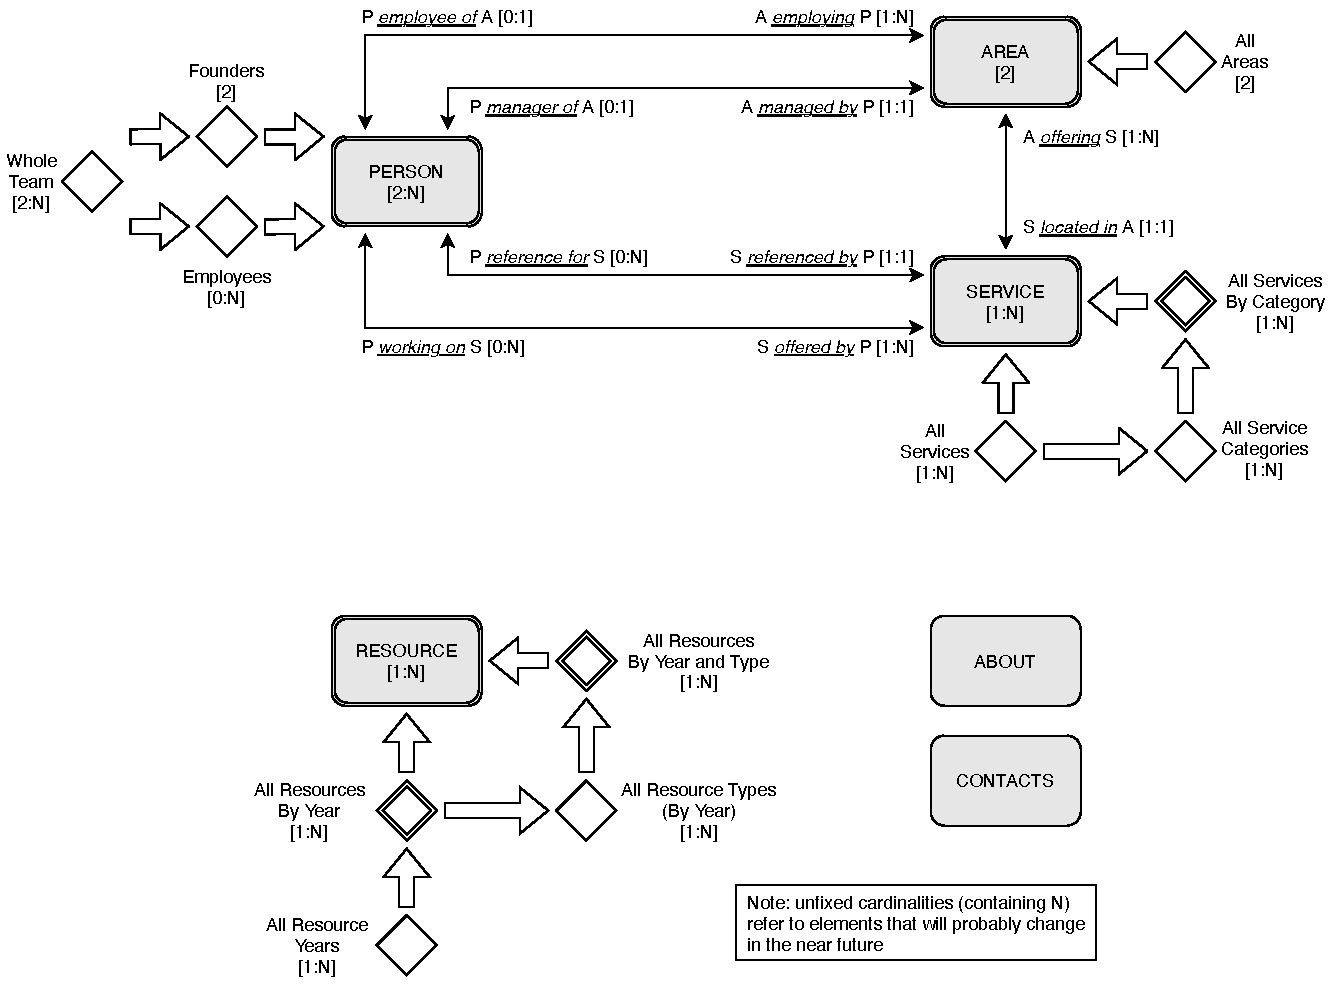
\includegraphics[width=\textwidth]{C-IDM.pdf}
	\caption{C-IDM Diagram}
\end{figure}

\chapter{Content tables}

%\chapter{Mapping Content Tables into Pages}

\chapter{P-IDM diagram}

\chapter{Visual Design}

\chapter{Interaction Scenarios}

\chapter{DB Design}

\end{document}